\documentclass[a4paper]{jpconf}
\usepackage[utf8]{inputenc}
\usepackage{graphicx}
\usepackage{lmodern}
\bibliographystyle{iopart-num}


\begin{document}
\title{The Neutron Monitor Control Panel}

\author{O. García-Población$^{1,2}$, H. Ivanov$^2$, I. García-Tejedor$^{1,2}$,
J. J. Blanco$^{1,2}$, J. Medina$^{1,2}$, R. Gómez-Herrero$^{1,2}$, E.
Catalán$^{1,2}$ and D. Radchenko$^{2}$}

\address{$^1$ Space Research Group, University of Alcalá, Spain}
\address{$^2$ Castilla-La Mancha Neutron Monitor, Parque Tecnológico de Guadalajara, Spain}

\ead{oscar.gpoblacion@uah.es}

\begin{abstract}
    This work presents the current status and future plans of NMCP, a new
    software developed to aid the operator in typical station maintenance and
    configuration operations. This software is integrated with new the NOAS
    data acquisition system and can be accessed using a supported web browser.
    If features a visual inspection tool to help the operator to identify
    spikes in the data, trace the origin of the spike back to the raw readings
    of each counter tube and pressure reading, and mark the data as invalid in
    the Neutron Monitor Database if desired. The software also provide
    information about station operation status, some descriptive statistics
    about current data being recorded and, in the future, will provide an
    interface to configure station parameters.
\end{abstract}

\section{Introduction}

%% Aquí hay que hablar de:
%% NMDB data quality. The origin of the spikes. The revision mechanism at NMDB.
%% The need of controlling monitor operation and data. The data acquisition system and
%% how it is related with the operation of the station and its data quality.
Neutron Monitor data is widely used by researchers in different research fields not necessarily related with cosmic rays. That's why the NMBD
puts effort into delivering data with the best quality possible. The data is also used in real time GLE alarm systems and other real time
applications therefore the data quality protocol must be applied in real time. Eventually the data will be revised by a human supervisor to 
ensure the correct behaviour of the quality protocol. By quality protocol we refer to all the methods and techniques used such as:
\begin{itemize}
	\item   Detection of abnormal data, commonly referred as spikes.
	\item   Detection of inactivity which will lead to a notification to the team responsible for the neutron monitor station.
	\item   Monitor neutrons are usually formed by 18 counter tubes. A malfunction in a single tube won't affect the overall value measured
	  	by the neutron monitor but it's not something desirable. This leads us to the need of monitoring and detection of malfunctions
		separately in each of the tubes.  
	\item	Detection of changes regard of the historical activity. Instrumental changes or changes in the immediate environment can cause 
	  	overall changes in the measured values of a monitor neutron. Detecting and correcting those changes is desirable.
	\item 	Comparing the data from one NM station with the data of different nearby NM stations. Detecting isolated events in one NM
	  	station indicates us that there is a malfunction in that NM station.	
\end{itemize}
Once detected the corrupt data, most of the times it can be traced down to its cause. Most of the times those malfunctions are caused by the
instruments forming the data acquisition system. Detecting the corrupt data and its cause helps us to improve and learn more about the data
acquisition system. In order to make easier the detection of the corrupt data we are working in the development of a Web tool which will help
us detect the corrupted data. The Web application makes use of dynamically generated plots which aim to highlight possible corrupted data.


blabla \cite{Medina2013}
blabla \cite{NMDB2011}
blabla \cite{Forbush1938}

\section{System architecture}

There are two main roles in the architecture: a client that requests and
consumes data using a web browser, and a system that collects and serves the
data, which in this system is the data acquisition system\cite{Garcia2014}. This
separation of roles follows the client-server design
pattern\cite{wiki:ClientServer}.

The software architecture is based on the Model-View-Controller (MVC) software
design pattern\cite{wiki:MVC}. This pattern encourages the separation between
the data, the data processing and the data representation. 

The view component is in charge of the data representation and the user
interface. In our system, this component is mainly executed by the client in a
web browser. The browser is not only a convenient graphical output device but
also provides a way to interact with the user. In response to these
interactions, the browser makes requests to a server which answers back with new
data to be represented.

The model component is located on the server side, in the data acquisition
system. This model comprises all the data captured from each counter tube and
the algorithms used to process these data, such as atmospheric pressure
corrections, sanity controls, editors to combine all the readings into a single
one, etc.

\begin{figure}[h]
    \centering
    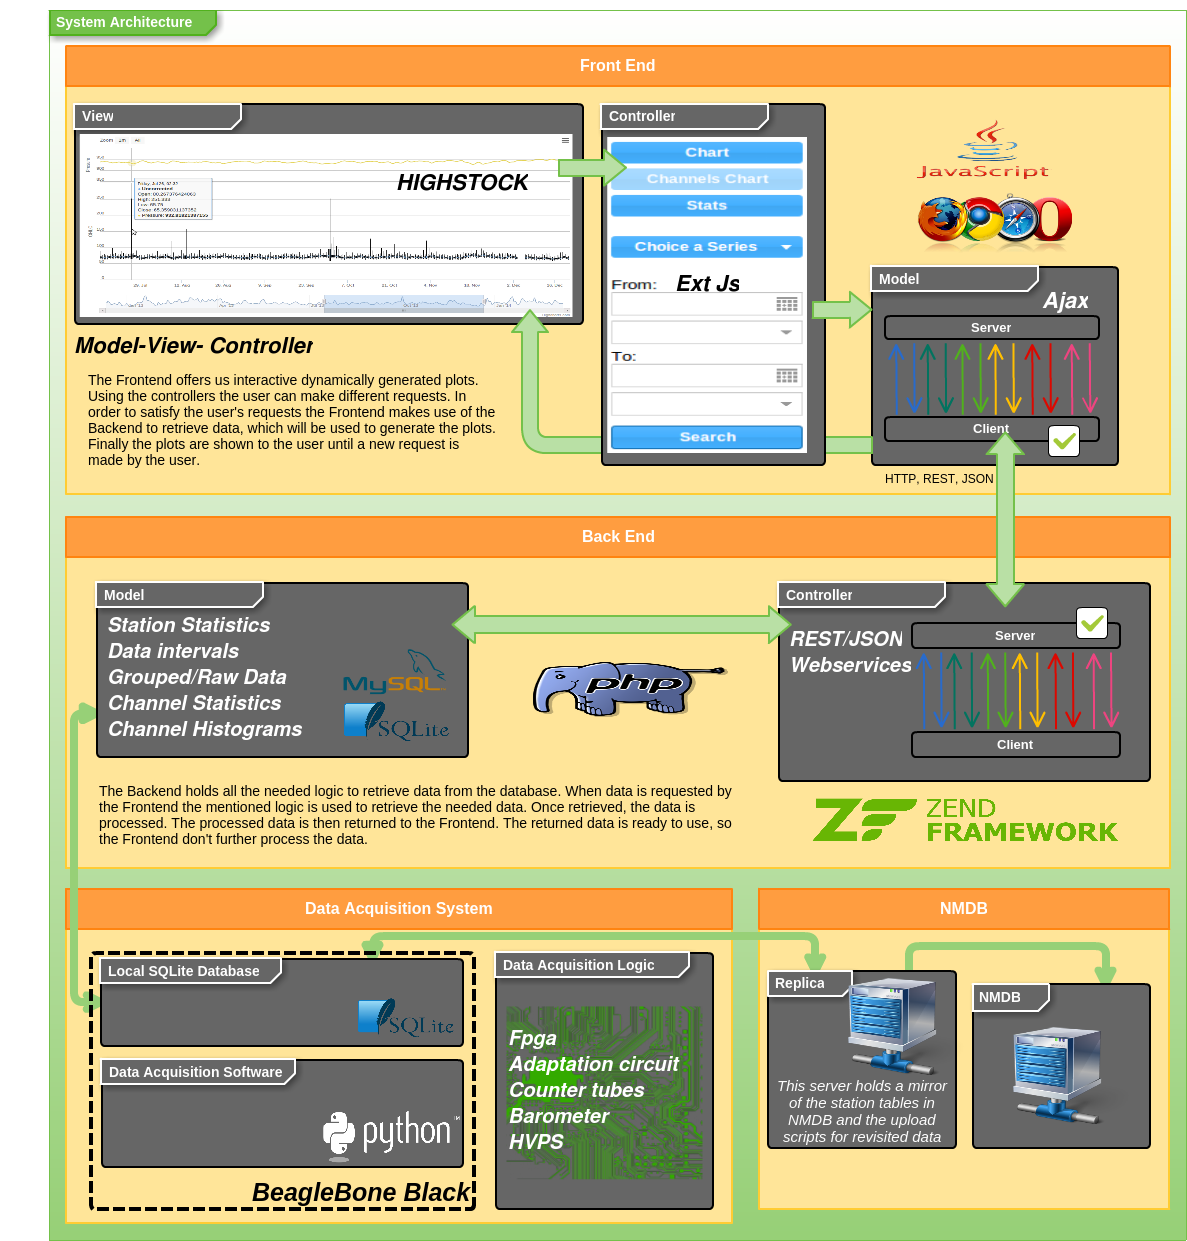
\includegraphics[keepaspectratio, width=1\textwidth]{./resources/Architecture.png}
    \caption{Architecture}
    \label{fig:arch}
\end{figure}

\section{The spike tool}
%% Aquí hablaremos concretamente del spike tool. Sobre todo de cómo funciona
%% cara al usuario.
Currently the Spike Tool consist of three modules Spike, SpikeCorrected and ChannelStats. Spike and SpikeCorrected are very similar, 
SpikeCorrected works with a different set of data and have some extra functionality.

The Spike module offers a highly interactive chart in which the spikes are easy to trace. Initially the chart displays a large set of
data, and some kind of data grouping is needed. Just averaging the data flattens the spikes. Candlestick chart is used to prevent the
problem formerly detailed, this way the max and min values can be easily distinguished. Eventually when a short interval of data is 
requested and no grouping is needed to display the data, the chart will automatically switch to line chart.

As mentioned above the chart is highly interactive. It offers a very intuitive zooming facility. Clicking and dragging through and 
interval of the chart will raise a zoom event. Depending of the drag direction, the event will be zoom In or zoom Out. The chart 
offers a navigator which allows us to navigate forward or backward. Datetime input fields are available too, those allows us plot a
specific time interval.

At first the uncorrected data is used to generate the charts, but we are given the chance to choose between Uncorrected, efficiency
and pressure corrected data. The atmospheric  pressure is also plotted, this help us to evaluate how the atmospheric pressure affects
the measurements of our Neutron Monitor station.

Once we have localized a spike we can see the raw reading of the counter tubes. This allow us identify better the spike. Due to the
fact that there is 18 channels this option is available only when no data grouping is needed.

As said the SpikeCorrected module is very similar to the Spike module which we've been explaining above. First of all, this module 
use diferent set of data. The Spike module use the raw data which proceeds from the data adquisition system. SpikeCorr use the 
revisited data. Clicking on data, marks the data. The marked data is stored in a grid which we can visualize later on a separate 
window. Eventually we can submit the marked data to the revisited set of data. This means that the mentioned data will be considered 
invalid and treated as void in the future.

The marking is done through clicking on the data we want to mark. Once marked, on the time axis a flag will be added, the flag will
make it easier visualize marked data. There is a grid which contains all the marked data. This grid is visualized on a separate
windows. The window can be hidden when not needed and shown when needed. In that window we can also find the submit button.

%%TODO add ChannelStats module

\begin{figure}[h]
    \centering
    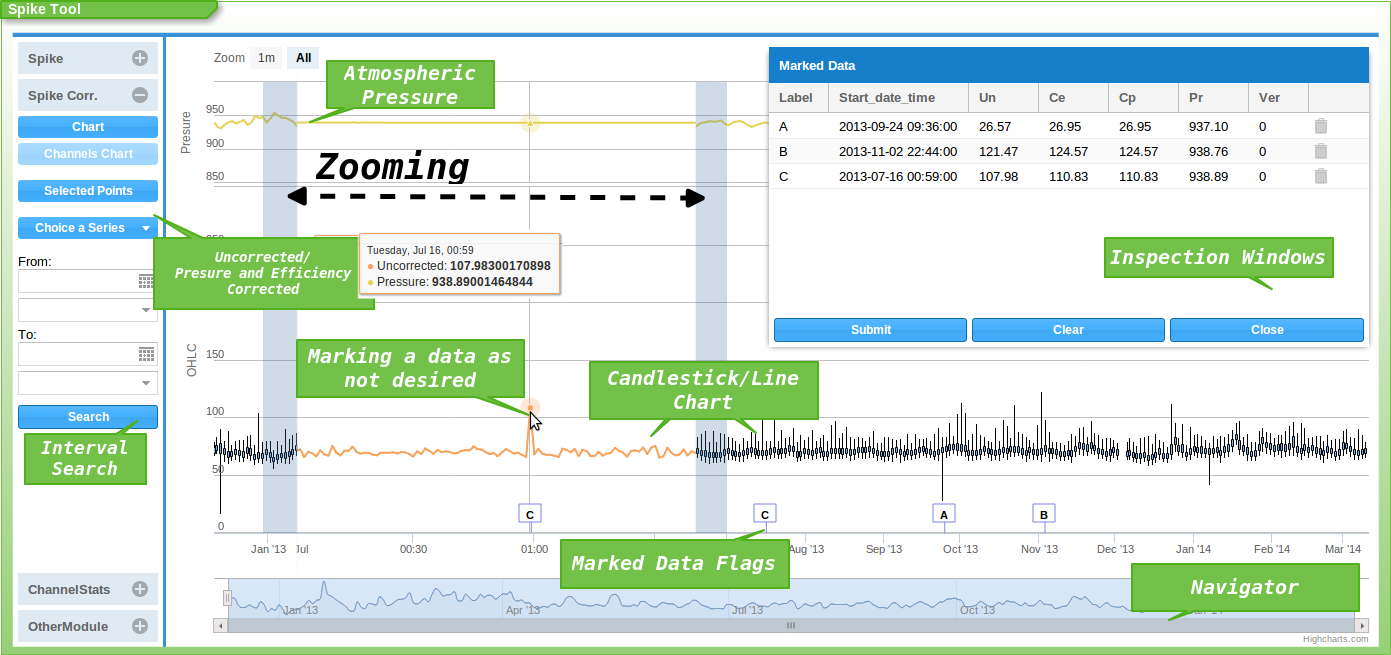
\includegraphics[keepaspectratio, width=1\textwidth]{./resources/SpikeTool.png}
    \caption{Spike Tool}
    \label{fig:arch}
\end{figure}

\section{Future work}

The neutron monitor control panel is a natural evolution of the new data
acquisition system designed for neutron monitors and it is under active
development to add new useful features in the near future. Some of these future
features are summarized bellow.

\begin{description}
    \item[Online statistics] The control panel will include a module for
        descriptive statistics that will be calculated in real time from the
        counter tubes raw readings. This will help to identify drifts in the
        behavior of the detectors and to apply the appropriate actions to
        maintain data quality.
    \item[Station reconfiguration] This will allow the operator to disconnect a
        counter from the station without affecting global station count. This
        can be useful to carry on maintenance operations such as counter tube
        diagnostics. 
    \item[Station parameter setup] New electronics allow the remote control of
        some parameters, for example the high voltage power supply set point,
        the remote database for data upload, backup policies, etc.
    \item[Alarms and push notifications] When connectivity allows it, it will
        be possible to configure alarms and notification to recipients using
        the new push mobile technologies, for example if the station is no
        longer uploading data to NMDB or if data is out of quality standards
    \item[Detector response histogram] A new design from the New
        Hampshire University of the front-end amplifiers provides a pulse which
        width is proportional to the energy of the incident particle. The new
        FPGA IP-core running in the NOAS, the second version of our data
        acquisition system, is able to read these pulses and to generate an
        histogram with the distribution of the pulses energy over a given time
        interval. This will enable a mechanism for non-intrusive diagnostics of
        the counter tubes. 
\end{description}


\subsection*{Acknowledgments} 
The authors would like to thank the OMNIweb team and the Neutron
Data Base for the use of their data. This work has been partially supported by
Ministerio de Ciencia y Tecnologia through the project AYA2012-39810-C02-01
Pic du Midi and Kiel.....



\section*{References}
\bibliography{iopart-num} 

\end{document}


